% !TEX root = ../sethomas_thesis_main.tex
\cleardoublepage
% \thispagestyle{empty}
\renewcommand{\chaptermark}[1]{\markboth{#1}{#1}}

\phantomsection
\addcontentsline{toc}{chapter}{Curriculum Vitae}
\chaptermark{Curriculum Vitae}
\pagenumbering{gobble}
\begin{center}
    \textbf{\Large Sean Thomas}\\
    Lausanne, Switzerland\\
    +41 79 780 4134\\
    seanthomas0409@gmail.com\\
    \href{http://www.sean-thomas.org}{sean-thomas.org}
\end{center}

\section*{About}
\hrulefill

\textbf{Technology and engineering} have always been my passion. During my \textbf{PhD}, I have learned that the best way to apply my creativity is in \textbf{research}. Being at the forefront of technology and
innovation is the ideal way to keep my creative juices flowing.

\section*{Education}
\hrulefill

\renewcommand{\arraystretch}{1}
\begin{tabular}{p{5cm}p{8.75cm}}
    September 2017 - January 2022 & \textbf{PhD in Robotics, Control and Intelligent Systems (Integrated Actuators Laboratory)}\\
    & Synthesis of Novel Integrated Actuators Powered by Shape Memory Alloys\\
    & Director : Prof. Yves Perriard\\
    September 2012 - March 2017 & \textbf{Master \& Bachelor of Science in Robotics and Autonomous Systems}\\
    & Polytechnic program with an emphasis on micro-engineering, robotics, autonomous control systems and sensors.
\end{tabular}

\section*{Publications}
\hrulefill

\begin{itemize}
    \setlength\itemsep{0em}
\item[] \textbf{S. Thomas}, L. Tissot-Daguette, et al., \textit{“Microgripper Device”}, European Patent Application, 21150579.7 - 1016\\
\item[] \textbf{S. Thomas}, P. Germano, T. Martinez, and Y. Perriard, \textit{“An untethered mechanically-intelligent inchworm robot powered by a shape memory alloy oscillator,”} Sensors and Actuators A: Physical, Dec. 2021\\
\newpage
\item[] \textbf{S. Thomas}, G. Maquignaz, A. Thabuis, and Y. Perriard, \textit{“A Self-Biasing Shape Memory Alloy Gripper for Lightweight Applications,”} in 2021 IEEE/RSJ International Conference on Intelligent Robots and Systems (IROS 2021), Sep. 2021\\
\item[] \textbf{S. Thomas}, A. Thabuis, T. Martinez, P. Germano, and Y. Perriard, \textit{“Designing compliant mechanisms composed of shape memory alloy and actuated by induction heating,”} Smart Mater. Struct., Aug. 2021\\
\item[] \textbf{S. Thomas}, P. Germano, T. Martinez, and Y. Perriard, \textit{“Control-Free Mechanical Oscillator Powered by Shape Memory Alloys,”} in 2021 IEEE/ASME International Conference on Advanced Intelligent Mechatronics (AIM), Jul. 2021\\
\item[] P. Peralta, \textbf{S. Thomas}, and Y. Perriard, \textit{“Characterization and Verification of Eddy-Current Position Sensing for Magnetic Levitation,”} IEEE Transactions on Industry Applications, 2021\\
\item[] \textbf{S. Thomas}, A. Thabuis, T. Martinez, and Y. Perriard, \textit{“Shape Memory Effect of Benchmark Compliant Mechanisms Designed With Topology Optimization,”} in 2020 IEEE/ASME International Conference on Advanced Intelligent Mechatronics (AIM), Jul. 2020\\
\item[] \textbf{S. Thomas}, A. Thabuis, T. Martinez, and Y. Perriard, \textit{“Multi-Output Compliant Shape Memory Alloy Bias-Spring Actuators,”} in 2020 IEEE/ASME International Conference on Advanced Intelligent Mechatronics (AIM), Jul. 2020\\
\item[] P. Peralta, \textbf{S. Thomas}, and Y. Perriard, \textit{“Integrated, Eddy-Current-Based Sensing of Rotor Position for Magnetic Levitation,”} in 2020 IEEE Energy Conversion Congress and Exposition (ECCE), Oct. 2020\\
\item[] \textbf{S. Thomas}, M. Almanza, and Y. Perriard, \textit{“Design Analysis of a Shape Memory Alloy Bias-Spring Linear Actuator,”} in 2019 12th International Symposium on Linear Drives for Industry Applications (LDIA), Jul. 2019\\
\item[] \textbf{S. Thomas}, P. Peralta, R. Mottet, M. Lehmann, Y. Civet, and Y. Perriard, \textit{“Analysis and Reduction of Time Response in Thermally Activated Shape Memory Alloys,”} in 2018 21st International Conference on Electrical Machines and Systems (ICEMS), Oct. 2018\\
\item[] \textbf{S. Thomas}, M. Almanza, Y. Civet, and Y. Perriard, \textit{“Actuation Displacement Analysis of a Self-Switching Shape Memory Alloy Buckled Beam,”} in 2018 21st International Conference on Electrical Machines and Systems (ICEMS), Oct. 2018\\
\item[] \textbf{S. Thomas}, L. Tissot-Daguette, T. Martinez, C. Baur, and Y. Perriard, \textit{“Design and Modelling of a Flexure-based Bistable Gripper Powered by Shape Memory Alloys,”} Sensors and Actuators A: Physical, 2022 (pending)
\end{itemize}

\section*{Experience}
\hrulefill

\begin{tabular}{p{5cm}p{8.75cm}}
    October 2016 - March 2017 & \textbf{Master Thesis at Human Robotics Group, Imperial College London} - Development of Single-Joint Neuromechanics device\\
    % & Development of a patient-specific exoskeleton system capable of measuring the joint impedance of motor-impaired patients. (\url{https://www.imperial.ac.uk/human-robotics})\\
    & Supervisors : Prof. Etienne Burdet; Prof. Hannes Bleuler; Dr. Mohamed Bouri; Dr. Hsien Yung Huang\\
    July 2016 - October 2016 & \textbf{Onward} - Human Rehabilitation Robot, R\&D engineer internship\\
    % & The project consisted of the design of the Human Rehabilitation Robot (JANE) and its implementation at the CRR Suva rehabilitation clinic.\\
    & Supervisors: Dr. Joachim v. Zitzewitz; Dr. Urs Keller\\
    July 2015 - March 2016 & \textbf{G-Lab, EPFL} - Sensor Design of Body Weight Support Robot for Rodent Rehabilitation\\
    % & The goal of this project consisted of the design and fabrication of a sensor to track the movement of motor-impaired rodents for a bodyweight support robot for rodent rehabilitation. The project involved sensor design, signal processing and flexure-based structures.\\
    & Supervisors: Prof. Gregoire Courtine; Dr. Joachim v. Zitzewitz
\end{tabular}

\section*{Skills}
\hrulefill

Python, C++, Objective C, Javascript, Java, HTML CSS, Matlab, 3D CAD, Finite Element Modelling, 3D Printing, Optimisation, LabView, Sensor Design, Modelling, Actuator Design, Latex
% \ifpdf
% 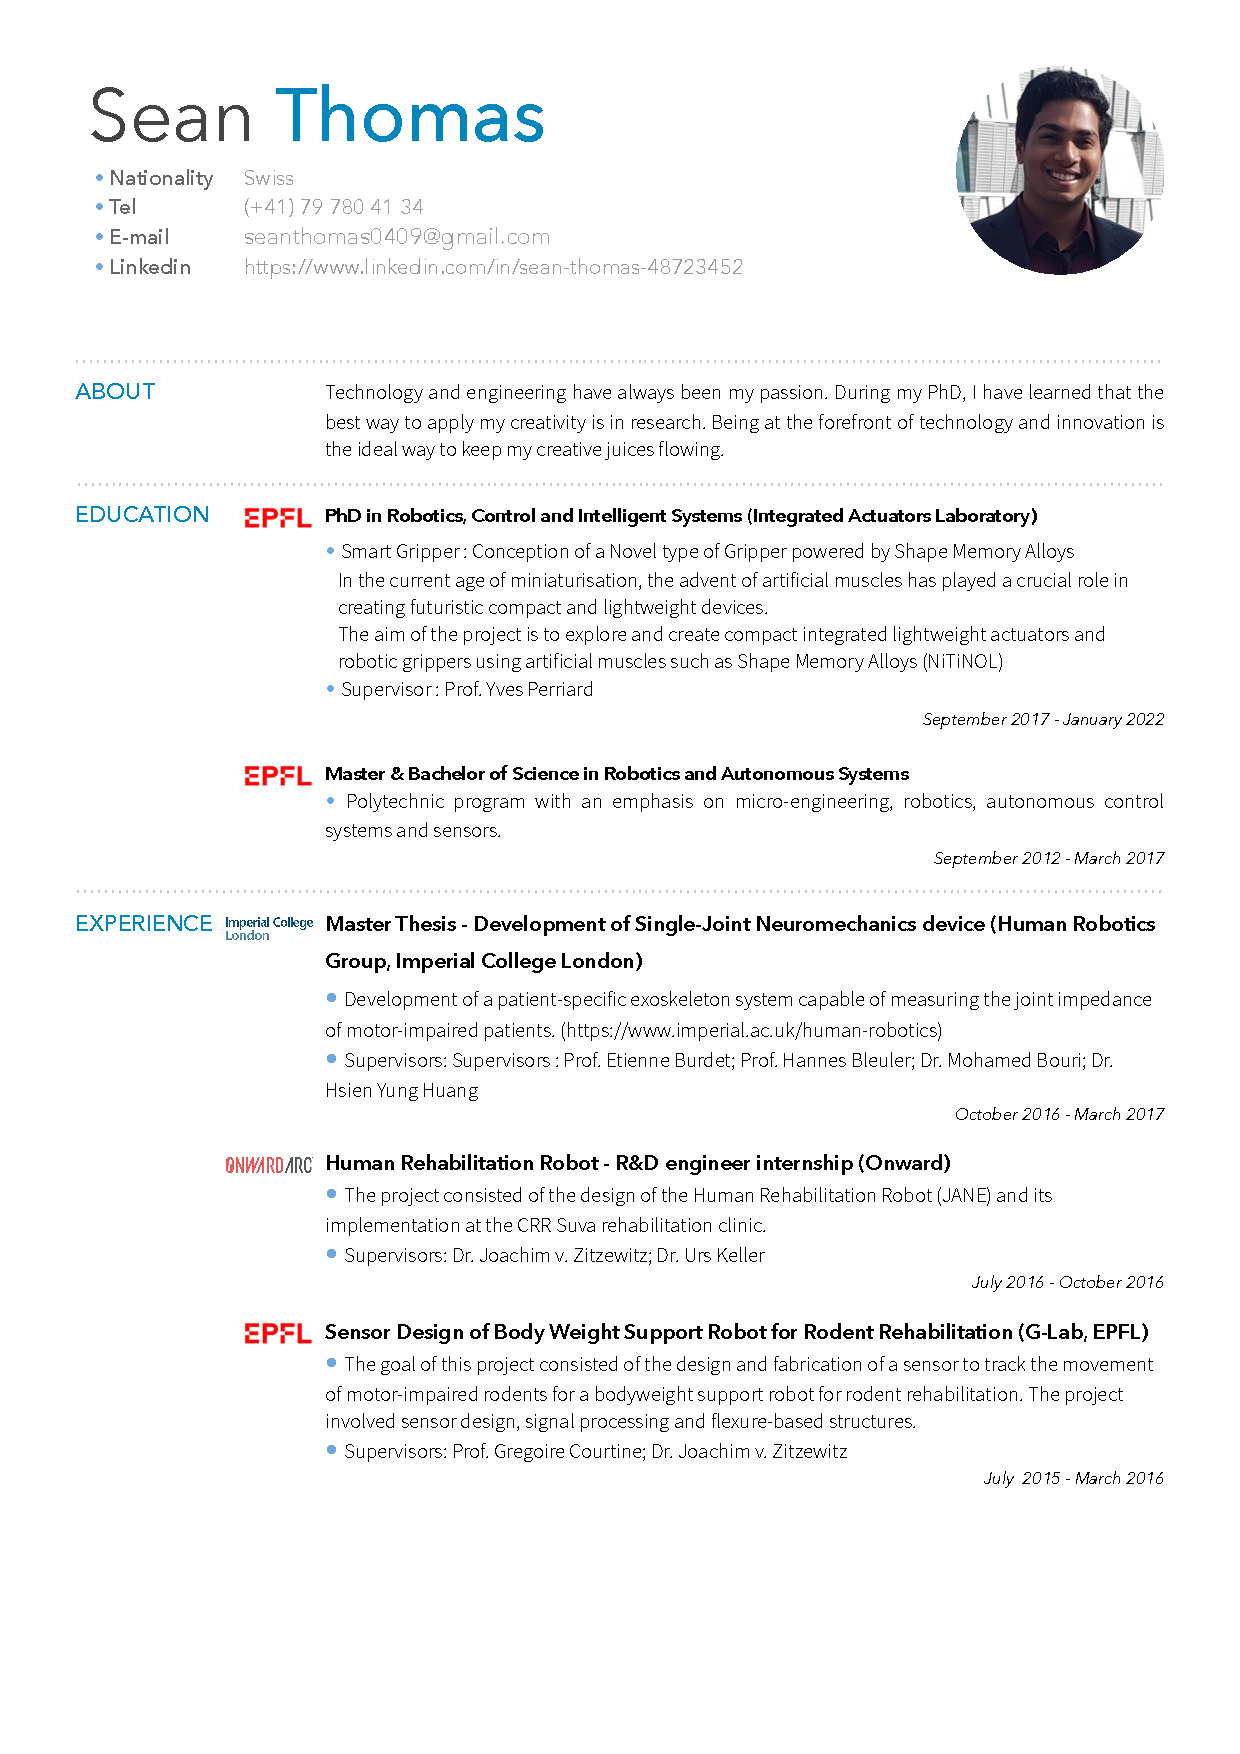
\includepdf[pagecommand=\thispagestyle{addpagenumbersforpdfimports},pages=-]{tail/seanthomas-cv.pdf}
% \fi
